\section{Entropy and Information for Spike Trains}
\label{sec:Entropy and Information for Spike Trains}


\begin{rem}
  Computing the entropy or information content of a neuronal response characterized by spike times is much more difficult than computing these quantities for responses described by firing rates. Nevertheless, these computations are important, because firing rates are incomplete descriptions that can lead to serious underestimates of the entropy and information.
\end{rem}

\begin{fac}
  \label{fac:spikeTrainInformation}
  Spike-train entropy calculations are typically based on the study of long-duration recordings consisting of many action potentials. The longer the total length of a spike train, the more information it contains.
\end{fac}

\begin{rem}
  By Fact \ref{fac:spikeTrainInformation}, the entropy and mutual information of spike trains are reported as entropy or information rates.
\end{rem}

\begin{defn}
  \label{def:entropyInformationRates}
  The \emph{entropy rate} and \emph{information rate} are defined as the total entropy and information divided by the duration of the spike train, respectively. Alternatively, entropy and mutual information can be divided by the total number of action potentials and reported as bits per spike rather than bits per second.
\end{defn}

\begin{ntn}
  We write the entropy rate as $\dot{H}$ rather than $H$.
\end{ntn}

\begin{fac}
  The temporal pattern of a group of action potentials can be specified by listing either the individual spike times or the sequence of intervals between successive spikes.
\end{fac}

\begin{rem}
  The entropy and mutual information calculations we present are based on a spike-time description, but as an initial example we consider an approximate computation of entropy using interspike intervals.
\end{rem}
\subsection{Based on Interspike Intervals}
\begin{rem}
  The interspike interval is a continuous variable.
\end{rem}
\begin{ntn}
  The probability of an interspike interval falling in the range between $\tau$ and $\tau+\Delta\tau$ is given in terms of the interspike interval probability density by $p[\tau]\Delta\tau$, where $\Delta\tau$ is the resolution.
\end{ntn}

\begin{prop}
  \label{prop:independentInterspike}
  If the different interspike intervals are statistically independent and identically distributed, the entropy associated with the interspike intervals in a spike train of average rate $\left<r\right>$ and of duration $T$ is
  \begin{displaymath}
    H = -\left<r\right>T\int_0^{\infty}p[\tau]\log_2(p[\tau]\Delta\tau)d\tau,
  \end{displaymath}
  where $\left<r\right>T$ is the number of intervals. In this case, the entropy rate is
  \begin{displaymath}
    \dot{H} = -\left<r\right>\int_0^{\infty}p[\tau]\log_2(p[\tau]\Delta\tau)d\tau.
  \end{displaymath}
\end{prop}
\begin{proof}
  These are directly from definitions of the entropy and entropy rate.
\end{proof}

\begin{exm}
  If a spike train is described by a homogeneous Poisson process with rate $\left<r\right>$, we have
  \begin{displaymath}
    p[\tau] = \left<r\right>e^{-\left<r\right>\tau}
  \end{displaymath}
  and the interspikes are statistically independent (Chapter \ref{cha:Neural Encoding I}). Thus,
  \begin{equation}
    \label{equ:4.53}
    \dot{H} = \frac{\left<r\right>}{\ln 2}(1-\ln\left<r\right>\Delta\tau).
  \end{equation}
  In fact,
  \begin{displaymath}
    \begin{aligned}
      \dot{H} &= -\left<r\right>\int_0^{\infty}\left<r\right>e^{-\left<r\right>\tau}\log_2(\left<r\right>e^{-\left<r\right>\tau}\Delta\tau)d\tau\\
      &= -\left<r\right>\int_0^{\infty}e^{-\tau}\log_2(\left<r\right>e^{-\tau}\Delta\tau)d\tau\\
      &= -\left<r\right>\left(\log_2(\left<r\right>\Delta\tau) + \int_0^{\infty}\frac{-e^{-\tau}}{\ln 2}d\tau\right) \\
      &= \frac{\left<r\right>}{\ln 2}(1-\ln\left<r\right>\Delta\tau),
    \end{aligned}
  \end{displaymath}
  where the second step follows from the variable substitution $\tau = \left<r\right> \tau$ and the third step from the integration by parts.
\end{exm}

\begin{defn}
  \label{PossionEntropyRate}
  Equation \ref{equ:4.53} is called the \emph{Poisson entropy rate}.
\end{defn}

\begin{thm}
  In general, the entropy rate $\dot{H}$ for a spike train with interspike interval distribution $p[\tau]$ and average rate $\left<r\right>$ satisfies
  \begin{equation}
    \label{equ:4.52}
    \dot{H} \leq -\left<r\right>\int_0^{\infty}p[\tau]\log_2(p[\tau]\Delta\tau)d\tau.
  \end{equation}
\end{thm}
\begin{proof}
  Correlations between different interspike intervals reduce the total entropy, so the result obtained by assuming independent intervals provides an upper bound on the true entropy of a spike train.
\end{proof}

\subsection{General Computations}

\begin{frm}
  To make entropy calculations practical, a long spike train is broken into statistically independent subunits, and the total entropy is written as the sum of the entropies for the individual subunits.
\end{frm}

\begin{exm}
  In the case of Proposition \ref{prop:independentInterspike}, the subunit was the interspike interval.
\end{exm}

\begin{rem}
  If interspike intervals are not independent, and we wish to compute a result and not merely a bound, we must work with larger subunit descriptions.
\end{rem}

\begin{ntn}
  The variable $T_s$ is used below to denote the duration of the spike sequence being considered, while $T$, which is much larger than $T_s$, is the duration of the entire spike train.
\end{ntn}

\begin{frm}
  Denote these basic subunits by spike sequences of duration $T_s$. A spike sequence can be obtained as follows.
  \begin{enumerate}[(i)]
  \item Divide time $T_{s}$ into discrete bins of size $\Delta t$, which is small enough so that not more than one spike appears in a bin.
  \item Label each bin by a 0 (no spike) or a 1 (spike), depending on whether or not a spike occurred within it.
  \item Represent a spike sequence defined over a block of duration $T_s$ by a string of $T_s/\Delta t$ zeros and ones.
  \end{enumerate}
  We denote such a sequence by $B(t)$, where $B$ is a $T_s/\Delta t$ bit binary number, and $t$ specifies the time of the first bin in the sequence being considered. Both $T_s$ and $t$ are integer multiples of the bin size $\Delta t$.
\end{frm}

\begin{ntn}
  The probability of a sequence $B$ occurring at any time during the entire response is denoted by $P[B]$.
\end{ntn}

\begin{rem}
  $P[B]$ can be obtained by counting the number of times the sequence $B$ occurs anywhere within the spike trains being analyzed (\emph{including overlapping cases}).
\end{rem}

\begin{prop}
  The spike-train entropy rate implied by the distribution that is characterized by $P[B]$ is
  \begin{equation}
    \label{equ:4.54}
    \dot{H} = -\frac{1}{T_{s}}\sum\limits_{B}P[B]\log_{2}P[B],
  \end{equation}
  where the sum is over all the sequences $B$ found in the data set, and we have divided by the duration $T_{s}$ of a single sequence to obtain an entropy rate.
\end{prop}
%\begin{proof}
 % Here $B$ is a possible value of the sequence over a block of duration $T_{s}$, which is the only one random variable involved.
%\end{proof}

\begin{prop}
  If the spike sequences in nonoverlapping intervals of duration $T_{s}$ are independent and identically distributed, the full spike-train entropy rate is also given by Equation \ref{equ:4.54}.
\end{prop}
\begin{proof}
  By the independence,
  \begin{displaymath}
    \begin{aligned}
      \dot{H} &= \frac{-T/T_{s}\sum\limits_{B}P[B]\log_{2}P[B]}{T} \\
      &= -\frac{1}{T_{s}}\sum\limits_{B}P[B]\log_{2}P[B],
    \end{aligned}
  \end{displaymath}
  which completes the proof.
\end{proof}

\begin{thm}
  For small $T_{s}$ such that the spike sequences are not independent, Equation \ref{equ:4.54} provides an upper bound on the true entropy rate, that is,
  \begin{equation}
    \label{eq:upper1}
    \dot{H} \leq -\frac{1}{T_{s}}\sum\limits_{B}P[B]\log_{2}P[B].
  \end{equation}
\end{thm}
\begin{proof}
  Any correlations between successive intervals (if $B(t+T_{s})$ is correlated with $B(t)$, for example) reduce the total spike-train entropy, causing Equation \ref{equ:4.54} to overestimate the true entropy rate.
\end{proof}

\begin{rem}
  If $T_{s}$ is too small, $B(t+T_{s})$ and $B(t)$ are likely to be correlated, and the overestimate may be severe. As $T_{s}$ increases, we expect the correlations to get smaller, and Equation \ref{equ:4.54} should provide a more accurate value.
\end{rem}

\begin{rem}
  For any finite data set, $T_{s}$ cannot be increased past a certain point, because there will not be enough spike sequences of duration $T_{s}$ in the data set to determine their probabilities. Thus, in practice, $T_{s}$ must be increased until the point where the extraction of probabilities becomes problematic, and some form of extrapolation to $T_{s}\to\infty$ must be made.
\end{rem}

\begin{asm}
  \label{asm:finite-true-relationship}
  Statistical mechanics arguments suggest that the difference between the entropy rate for finite $T_{s}$ and the true entropy rate for $T_{s}\to\infty$ should be proportional to $1/T_{s}$ for large $T_{s}$.
\end{asm}

\begin{prop}
  The true entropy rate can be estimated by linearly extrapolating a plot of the entropy rate versus $1/T_{s}$ to the point $1/T_{s} = 0$.
\end{prop}
\begin{proof}
  This is directly from Assumption \ref{asm:finite-true-relationship}.
\end{proof}

\begin{rem}
  To compute the mutual information rate for a spike train, we must subtract the full noise entropy rate from the full spike-train entropy rate.
\end{rem}

\begin{ntn}
  $P[B(t)]$ is the probability of finding a given sequence $B$ at time $t$ within a set of spike trains obtained on trials using the same stimulus. In contrast, $P[B]$, used in the spike-train entropy rate calculation, is the probability of finding the sequence $B$ at any time within these trains.
\end{ntn}

\begin{lem}
  \label{lem:noiseEntropyRate-t}
  If the same stimulus is used in repeated trials, the noise entropy rate at time $t$ satisfies
  \begin{displaymath}
    \dot{H}_{t} = -\frac{1}{T_{s}}\sum\limits_{B}P[B(t)]\log_{2}P[B(t)].
  \end{displaymath}
\end{lem}
\begin{proof}
  %Definition \ref{def:noiseEntropyRate-t} makes sense.
  The noise entropy rate is determined from the probabilities of finding various sequences $B$, given that they were evoked by the same stimulus. %This is done by considering sequences $B(t)$ that start at a fixed time $t$.
  If the same stimulus is used in repeated trials, sequences $B(t)$ that begin at time $t$ in every trial are generated by the same stimulus. Therefore, the conditional probability of the response, given the stimulus, is in this case the distribution $P[B(t)]$ for response sequences beginning at time $t$. This is obtained by determining the fraction of trials on which $B(t)$ was evoked.
\end{proof}

\begin{rem}
  Determining $P[B(t)]$ for a sufficient number of spike sequences may take a large number of trials using the same stimulus.
\end{rem}

\begin{prop}
  \label{prop:fullNoiseEntropyRate}
  The full noise entropy rate can be computed by averaging the noise entropy rate at time $t$ over all $t$ values, that is,
  \begin{equation}
    \label{equ:4.55}
    \dot{H}_{noise} = -\frac{\Delta t}{T}\sum\limits_{t}\left(\frac{1}{T_{s}}\sum\limits_{B}P[B(t)]\log_{2}P[B(t)]\right),
  \end{equation}
  where $T/\Delta t$ is the number of different $t$ values being summed.
\end{prop}
\begin{proof}
  In this case, the average over $t$ plays the role of the average over stimuli in Equation \ref{equ:4.6}. Then, Lemma \ref{lem:noiseEntropyRate-t} completes the proof.
\end{proof}

\begin{thm}
  If Equation \ref{equ:4.55} is based on finite-length spike sequences, it provides an upper bound on the noise entropy rate, that is,
  \begin{equation}
    \label{equ:upper2}
    \dot{H}_{noise} \leq -\frac{\Delta t}{T}\sum\limits_{t}\left(\frac{1}{T_{s}}\sum\limits_{B}P[B(t)]\log_{2}P[B(t)]\right).
  \end{equation}
\end{thm}

\begin{prop}
  The true noise entropy rate is estimated by performing a linear extrapolation in $1/T_s$ to $1/T_s = 0$.
\end{prop}
\begin{proof}
  As was done for the spike-train entropy rate.
\end{proof}

\begin{exm}
  Entropy and noise entropy rates for the H1 visual neuron in the fly responding to a randomly moving visual image are shown in the following picture. (i) The filled circles in the upper trace show the full spike-train entropy rate computed for different values of $1/T_s$. The straight line is a linear extrapolation to $1/T_s = 0$, which corresponds to $T_s\to \infty$. (ii) The lower trace shows the spike train noise entropy rate for different values of $1/T_s$. The straight line is again an extrapolation to $1/T_s = 0$.
  \begin{center}
    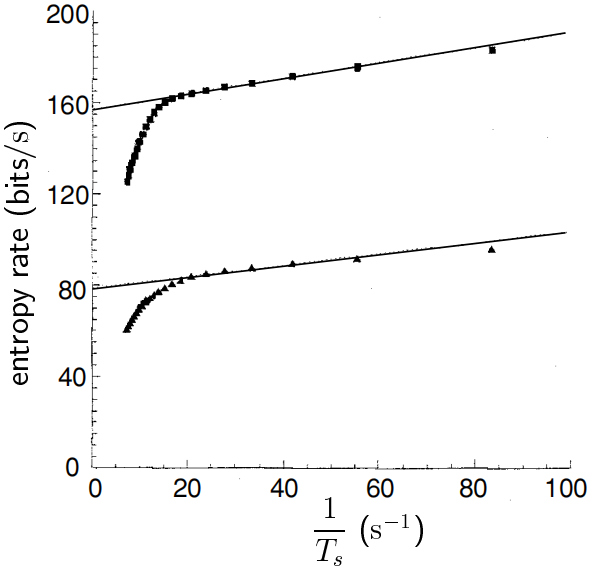
\includegraphics[scale=0.45]{./png/entropyRateEst}
  \end{center}
  Both entropy rates increase as functions of $1/T_s$, and the true spike-train and noise entropy rates are overestimated at large values of $1/T_s$. At $1/T_s\approx 20/s$, there is a sudden shift in the dependence. This occurs when there is insufficient data to compute the spike sequence probabilities. 
  % The difference between the $y$ intercepts of the two straight lines plotted is the mutual information rate.
  By linearly extrapolating the linear part of the series of computed points spike trains had an approximate entropy rate of 157 bits/s and an appeoximate noise entropy rate of 79 bits/s when the resolution was $\Delta t = 3$ ms. The information rate is obtained by taking the difference between the extrapolated values for the spiketrain and noise entropy rates. The result is an information rate of 157 - 79 = 78 bits/s or 1.8 bits/spike.
\end{exm}

\begin{rem}
  Both the spike-train and noise entropy rates depend on $\Delta t$. The leading dependence, coming from the $\log_{2}\Delta t$ term discussed previously, cancels in the computation of the information rate, but the information can still depend on $\Delta t$ through nondivergent terms. This reflects the fact that more information can be extracted from accurately measured spike times than from poorly measured spike times. Thus, we expect the information rate to increase with decreasing $\Delta t$, at least over some range of $\Delta t$ values.  At some critical value of $\Delta t$ that matches the natural degree of noise jitter in the spike timings, we expect the information rate to stop increasing. This value of $\Delta t$ is interesting because it tells us about the degree of spike timing accuracy in neural encoding.
\end{rem}

\begin{rem}
  The information conveyed by spike trains can be used to compare responses to different stimuli and thereby reveal stimulus-specific aspects of neural encoding.
\end{rem}


 



%%% Local Variables:
%%% mode: latex
%%% TeX-master: "../notesOnFluidMechanics"
%%% End:
